% Options for packages loaded elsewhere
\PassOptionsToPackage{unicode}{hyperref}
\PassOptionsToPackage{hyphens}{url}
%
\documentclass[
]{book}
\usepackage{amsmath,amssymb}
\usepackage{lmodern}
\usepackage{ifxetex,ifluatex}
\ifnum 0\ifxetex 1\fi\ifluatex 1\fi=0 % if pdftex
  \usepackage[T1]{fontenc}
  \usepackage[utf8]{inputenc}
  \usepackage{textcomp} % provide euro and other symbols
\else % if luatex or xetex
  \usepackage{unicode-math}
  \defaultfontfeatures{Scale=MatchLowercase}
  \defaultfontfeatures[\rmfamily]{Ligatures=TeX,Scale=1}
\fi
% Use upquote if available, for straight quotes in verbatim environments
\IfFileExists{upquote.sty}{\usepackage{upquote}}{}
\IfFileExists{microtype.sty}{% use microtype if available
  \usepackage[]{microtype}
  \UseMicrotypeSet[protrusion]{basicmath} % disable protrusion for tt fonts
}{}
\makeatletter
\@ifundefined{KOMAClassName}{% if non-KOMA class
  \IfFileExists{parskip.sty}{%
    \usepackage{parskip}
  }{% else
    \setlength{\parindent}{0pt}
    \setlength{\parskip}{6pt plus 2pt minus 1pt}}
}{% if KOMA class
  \KOMAoptions{parskip=half}}
\makeatother
\usepackage{xcolor}
\IfFileExists{xurl.sty}{\usepackage{xurl}}{} % add URL line breaks if available
\IfFileExists{bookmark.sty}{\usepackage{bookmark}}{\usepackage{hyperref}}
\hypersetup{
  pdftitle={Reticular Action Model (RAM) Notation Notes},
  pdfauthor={Ivan Jacob Agaloos Pesigan},
  hidelinks,
  pdfcreator={LaTeX via pandoc}}
\urlstyle{same} % disable monospaced font for URLs
\usepackage{color}
\usepackage{fancyvrb}
\newcommand{\VerbBar}{|}
\newcommand{\VERB}{\Verb[commandchars=\\\{\}]}
\DefineVerbatimEnvironment{Highlighting}{Verbatim}{commandchars=\\\{\}}
% Add ',fontsize=\small' for more characters per line
\usepackage{framed}
\definecolor{shadecolor}{RGB}{248,248,248}
\newenvironment{Shaded}{\begin{snugshade}}{\end{snugshade}}
\newcommand{\AlertTok}[1]{\textcolor[rgb]{0.94,0.16,0.16}{#1}}
\newcommand{\AnnotationTok}[1]{\textcolor[rgb]{0.56,0.35,0.01}{\textbf{\textit{#1}}}}
\newcommand{\AttributeTok}[1]{\textcolor[rgb]{0.77,0.63,0.00}{#1}}
\newcommand{\BaseNTok}[1]{\textcolor[rgb]{0.00,0.00,0.81}{#1}}
\newcommand{\BuiltInTok}[1]{#1}
\newcommand{\CharTok}[1]{\textcolor[rgb]{0.31,0.60,0.02}{#1}}
\newcommand{\CommentTok}[1]{\textcolor[rgb]{0.56,0.35,0.01}{\textit{#1}}}
\newcommand{\CommentVarTok}[1]{\textcolor[rgb]{0.56,0.35,0.01}{\textbf{\textit{#1}}}}
\newcommand{\ConstantTok}[1]{\textcolor[rgb]{0.00,0.00,0.00}{#1}}
\newcommand{\ControlFlowTok}[1]{\textcolor[rgb]{0.13,0.29,0.53}{\textbf{#1}}}
\newcommand{\DataTypeTok}[1]{\textcolor[rgb]{0.13,0.29,0.53}{#1}}
\newcommand{\DecValTok}[1]{\textcolor[rgb]{0.00,0.00,0.81}{#1}}
\newcommand{\DocumentationTok}[1]{\textcolor[rgb]{0.56,0.35,0.01}{\textbf{\textit{#1}}}}
\newcommand{\ErrorTok}[1]{\textcolor[rgb]{0.64,0.00,0.00}{\textbf{#1}}}
\newcommand{\ExtensionTok}[1]{#1}
\newcommand{\FloatTok}[1]{\textcolor[rgb]{0.00,0.00,0.81}{#1}}
\newcommand{\FunctionTok}[1]{\textcolor[rgb]{0.00,0.00,0.00}{#1}}
\newcommand{\ImportTok}[1]{#1}
\newcommand{\InformationTok}[1]{\textcolor[rgb]{0.56,0.35,0.01}{\textbf{\textit{#1}}}}
\newcommand{\KeywordTok}[1]{\textcolor[rgb]{0.13,0.29,0.53}{\textbf{#1}}}
\newcommand{\NormalTok}[1]{#1}
\newcommand{\OperatorTok}[1]{\textcolor[rgb]{0.81,0.36,0.00}{\textbf{#1}}}
\newcommand{\OtherTok}[1]{\textcolor[rgb]{0.56,0.35,0.01}{#1}}
\newcommand{\PreprocessorTok}[1]{\textcolor[rgb]{0.56,0.35,0.01}{\textit{#1}}}
\newcommand{\RegionMarkerTok}[1]{#1}
\newcommand{\SpecialCharTok}[1]{\textcolor[rgb]{0.00,0.00,0.00}{#1}}
\newcommand{\SpecialStringTok}[1]{\textcolor[rgb]{0.31,0.60,0.02}{#1}}
\newcommand{\StringTok}[1]{\textcolor[rgb]{0.31,0.60,0.02}{#1}}
\newcommand{\VariableTok}[1]{\textcolor[rgb]{0.00,0.00,0.00}{#1}}
\newcommand{\VerbatimStringTok}[1]{\textcolor[rgb]{0.31,0.60,0.02}{#1}}
\newcommand{\WarningTok}[1]{\textcolor[rgb]{0.56,0.35,0.01}{\textbf{\textit{#1}}}}
\usepackage{longtable,booktabs,array}
\usepackage{calc} % for calculating minipage widths
% Correct order of tables after \paragraph or \subparagraph
\usepackage{etoolbox}
\makeatletter
\patchcmd\longtable{\par}{\if@noskipsec\mbox{}\fi\par}{}{}
\makeatother
% Allow footnotes in longtable head/foot
\IfFileExists{footnotehyper.sty}{\usepackage{footnotehyper}}{\usepackage{footnote}}
\makesavenoteenv{longtable}
\usepackage{graphicx}
\makeatletter
\def\maxwidth{\ifdim\Gin@nat@width>\linewidth\linewidth\else\Gin@nat@width\fi}
\def\maxheight{\ifdim\Gin@nat@height>\textheight\textheight\else\Gin@nat@height\fi}
\makeatother
% Scale images if necessary, so that they will not overflow the page
% margins by default, and it is still possible to overwrite the defaults
% using explicit options in \includegraphics[width, height, ...]{}
\setkeys{Gin}{width=\maxwidth,height=\maxheight,keepaspectratio}
% Set default figure placement to htbp
\makeatletter
\def\fps@figure{htbp}
\makeatother
\setlength{\emergencystretch}{3em} % prevent overfull lines
\providecommand{\tightlist}{%
  \setlength{\itemsep}{0pt}\setlength{\parskip}{0pt}}
\setcounter{secnumdepth}{5}
\usepackage{booktabs}
\usepackage{amsthm}
\usepackage[left = 1in,right = 1in,top = 1in, bottom = 1in]{geometry}
\makeatletter
\def\thm@space@setup{%
  \thm@preskip=8pt plus 2pt minus 4pt
  \thm@postskip=\thm@preskip
}
\makeatother
\ifluatex
  \usepackage{selnolig}  % disable illegal ligatures
\fi
\usepackage[]{natbib}
\bibliographystyle{apalike}

\title{Reticular Action Model (RAM) Notation Notes}
\author{Ivan Jacob Agaloos Pesigan}
\date{2021-01-18}

\usepackage{amsthm}
\newtheorem{theorem}{Theorem}[chapter]
\newtheorem{lemma}{Lemma}[chapter]
\newtheorem{corollary}{Corollary}[chapter]
\newtheorem{proposition}{Proposition}[chapter]
\newtheorem{conjecture}{Conjecture}[chapter]
\theoremstyle{definition}
\newtheorem{definition}{Definition}[chapter]
\theoremstyle{definition}
\newtheorem{example}{Example}[chapter]
\theoremstyle{definition}
\newtheorem{exercise}{Exercise}[chapter]
\theoremstyle{remark}
\newtheorem*{remark}{Remark}
\newtheorem*{solution}{Solution}
\begin{document}
\maketitle

{
\setcounter{tocdepth}{1}
\tableofcontents
}
\hypertarget{description}{%
\chapter{Description}\label{description}}

This is a collection of my personal notes on the Reticular Action Model (RAM) notation
that accompanies the \texttt{ramR} package \citep{R-ramR}.
You can install the released version of \texttt{ramR} from \href{https://github.com/jeksterslab/ramR}{GitHub} with:

\begin{Shaded}
\begin{Highlighting}[]
\NormalTok{remotes}\SpecialCharTok{::}\FunctionTok{install\_github}\NormalTok{(}\StringTok{"jeksterslab/ramR"}\NormalTok{)}
\end{Highlighting}
\end{Shaded}

These notes are based on the following resources:

\begin{itemize}
\tightlist
\item
  \citet{Boker-2005}
\item
  \citet{McArdle-1984}
\item
  \citet{McArdle-2005}
\end{itemize}

See \href{https://jeksterslab.github.io/ramR_notes/index.html}{GitHub Pages}
for the html deployment.

\hypertarget{ram-matrix-notation}{%
\chapter{Reticular Action Model (RAM) Matrix Notation}\label{ram-matrix-notation}}

\hypertarget{full-model}{%
\section{Full Model}\label{full-model}}

\begin{definition}
\protect\hypertarget{def:unnamed-chunk-2}{}{\label{def:unnamed-chunk-2} }\begin{equation}
  \mathbf{v}
  =
  \mathbf{A} \mathbf{v} + \mathbf{u}
\end{equation}
\end{definition}

\noindent where

\begin{itemize}
\tightlist
\item
  \(\mathbf{v}\) and \(\mathbf{u}\) are \(t \times 1\) vectors of random variables
\item
  \(\mathbf{A}\) is a \(t \times t\) matrix of \emph{directed} or \emph{asymmetric} relationship
  from column variable \(v_j\) to row variable \(v_i\)

  \begin{itemize}
  \tightlist
  \item
    \(\mathbf{A}\) represent the regression of each of the \(t\) variables \(\mathbf{v}\) on the other \(t - 1\) variables
  \item
    diagonal \(a_{i,i}\) is zero
  \item
    \(u_i\) represent the residual of \(v_i\)
  \item
    if all regression coefficients on other variables are zero,
    then the variable \(v_i\) is considered the same as its own residual \(u_i\)
  \end{itemize}
\end{itemize}

\begin{definition}
\protect\hypertarget{def:unnamed-chunk-3}{}{\label{def:unnamed-chunk-3} }\begin{equation}
  \mathbf{S}
  =
  \mathbb{E}
  \left\{
    \mathbf{u} \mathbf{u}^{\prime}
  \right\} ,
\end{equation}
\end{definition}

\noindent where

\begin{itemize}
\tightlist
\item
  \(\mathbf{S}\) is a \(t \times t\) matrix of \emph{undirected} or \emph{symmetric} relationship

  \begin{itemize}
  \tightlist
  \item
    the notation \(\boldsymbol{\Omega}\) is used in other sources for \(\mathbf{S}\)
  \end{itemize}
\item
  \(\mathbb{E}\) is the expectation operator
\end{itemize}

\begin{definition}
\protect\hypertarget{def:unnamed-chunk-4}{}{\label{def:unnamed-chunk-4} }\begin{equation}
  \mathbf{C}
  =
  \mathbb{E}
  \left\{
    \mathbf{v} \mathbf{v}^{\prime}
  \right\} ,
\end{equation}
\end{definition}

\noindent where

\begin{itemize}
\tightlist
\item
  \(\mathbf{C}\) is a \(t \times t\) variance-covariance matrix

  \begin{itemize}
  \tightlist
  \item
    the notation \(\boldsymbol{\Sigma}\) is used in other sources for \(\mathbf{C}\)
  \end{itemize}
\end{itemize}

\begin{definition}
\protect\hypertarget{def:unnamed-chunk-5}{}{\label{def:unnamed-chunk-5} }\begin{equation*}
  \mathbf{v}
  =
  \mathbf{A} \mathbf{v} + \mathbf{u}
\end{equation*}

\noindent can be rewritten as

\begin{equation}
  \begin{split}
    \mathbf{v} - \mathbf{A} \mathbf{v}
    &=
    \mathbf{u} \\
    \mathbf{u}
    &=
    \mathbf{v} - \mathbf{A} \mathbf{v} \\
    \mathbf{u}
    &=
    \left( \mathbf{I} - \mathbf{A} \right) \mathbf{v}
  \end{split}
\end{equation}

\noindent assuming that \(\left( \mathbf{I} - \mathbf{A} \right)\) is non-singular,

\begin{equation}
  \mathbf{E}
  = 
  \left( \mathbf{I} - \mathbf{A} \right)^{-1}
\end{equation}

\noindent then

\begin{equation}
  \begin{split}
    \mathbf{v}
    &=
    \left( \mathbf{I} - \mathbf{A} \right)^{-1} \mathbf{u} \\
    &=
    \mathbf{E} \mathbf{u} .
  \end{split}
\end{equation}
\end{definition}

Using the definitions above,
\(\mathbf{S}\) and \(\mathbf{C}\)
are given by

\begin{equation}
  \begin{split}
    \mathbf{S}
    &=
    \left( \mathbf{I} - \mathbf{A} \right)
    \mathbf{C}
    \left( \mathbf{I} - \mathbf{A} \right)^{-1} \\
    &=
    \mathbf{E}^{-1} \mathbf{C} \left( \mathbf{E}^{-1} \right)^{\mathsf{T}}
    \end{split}
\end{equation}

\begin{equation}
  \begin{split}
    \mathbf{C}
    &=
    \left( \mathbf{I} - \mathbf{A} \right)^{-1}
    \mathbf{S}
    \left[ \left( \mathbf{I} - \mathbf{A} \right)^{-1} \right]^{\mathsf{T}} \\
    &=
    \mathbf{E} \mathbf{S} \mathbf{E}^{\mathsf{T}}
  \end{split}
\end{equation}

\hypertarget{observedmanifestgiven-variables-vs.-unobservedlatenthidden-variables}{%
\section{Observed/Manifest/Given Variables vs.~Unobserved/Latent/Hidden Variables}\label{observedmanifestgiven-variables-vs.-unobservedlatenthidden-variables}}

\begin{definition}
\protect\hypertarget{def:unnamed-chunk-6}{}{\label{def:unnamed-chunk-6} }\begin{equation}
  \mathbf{v}
  =
  \begin{bmatrix}
    \mathbf{g}_{p \times 1} \\
    \mathbf{h}_{q \times 1} \\
  \end{bmatrix}
\end{equation}

\begin{equation}
  t = p + q
\end{equation}
\end{definition}

\begin{itemize}
\tightlist
\item
  \(\mathbf{g}\) may be considered observed, manifest or \emph{given} variables
\item
  \(\mathbf{h}\) may be considered unobserved, latent, or \emph{hidden} variables
\end{itemize}

\begin{definition}
\protect\hypertarget{def:unnamed-chunk-7}{}{\label{def:unnamed-chunk-7} }\begin{equation}
  \mathbf{F}
  =
  \begin{bmatrix}
    \mathbf{I}_{p \times p} : \mathbf{0}_{p \times q}
  \end{bmatrix}
\end{equation}
\end{definition}

\begin{itemize}
\tightlist
\item
  the \(\mathbf{F}\) matrix acts as a \emph{filter} to select the manifest variables
  out of the full set of manifest and latent variables
\end{itemize}

\begin{equation}
  \mathbf{g}
  =
  \mathbf{F}
  \mathbf{v}
\end{equation}

\begin{equation}
  \begin{split}
    \mathbf{g}
    &=
    \mathbf{F} \left( \mathbf{I} - \mathbf{A} \right)^{-1} \mathbf{u} \\
    &=
    \mathbf{F} \mathbf{E} \mathbf{u}
  \end{split}
\end{equation}

\begin{definition}
\protect\hypertarget{def:unnamed-chunk-8}{}{\label{def:unnamed-chunk-8} }\begin{equation}
  \mathbf{M}
  =
  \mathbb{E}
  \left\{
    \mathbf{g}
    \mathbf{g}^{\mathsf{T}}
  \right\}
\end{equation}
\end{definition}

\begin{equation}
  \begin{split}
    \mathbf{M}
    &=
    \mathbf{F}
    \left( \mathbf{I} - \mathbf{A} \right)^{-1}
    \mathbf{S}
    \left[ \left( \mathbf{I} - \mathbf{A} \right)^{-1} \right]^{\mathsf{T}}
    \mathbf{F}^{\mathsf{T}} \\
    &=
    \mathbf{F}
    \mathbf{E} \mathbf{S} \mathbf{E}^{\mathsf{T}}
    \mathbf{F}^{\mathsf{T}} \\
    &=
    \mathbf{F}
    \mathbf{C}
    \mathbf{F}^{\mathsf{T}}
  \end{split}
\end{equation}

\begin{itemize}
\tightlist
\item
  when components of \(\mathbf{v}\) are permuted,
  the columns of \(\mathbf{F}\) can be correspondingly permuted
\item
  the rows and columns of \(\mathbf{C}\) that are filtered out by \(\mathbf{F}\)
  contain useful information about the latent variable structure.
\end{itemize}

The equations above completely define RAM.

\hypertarget{ram-diagram}{%
\chapter{Reticular Action Model (RAM) Path Diagram}\label{ram-diagram}}

\begin{figure}
\centering
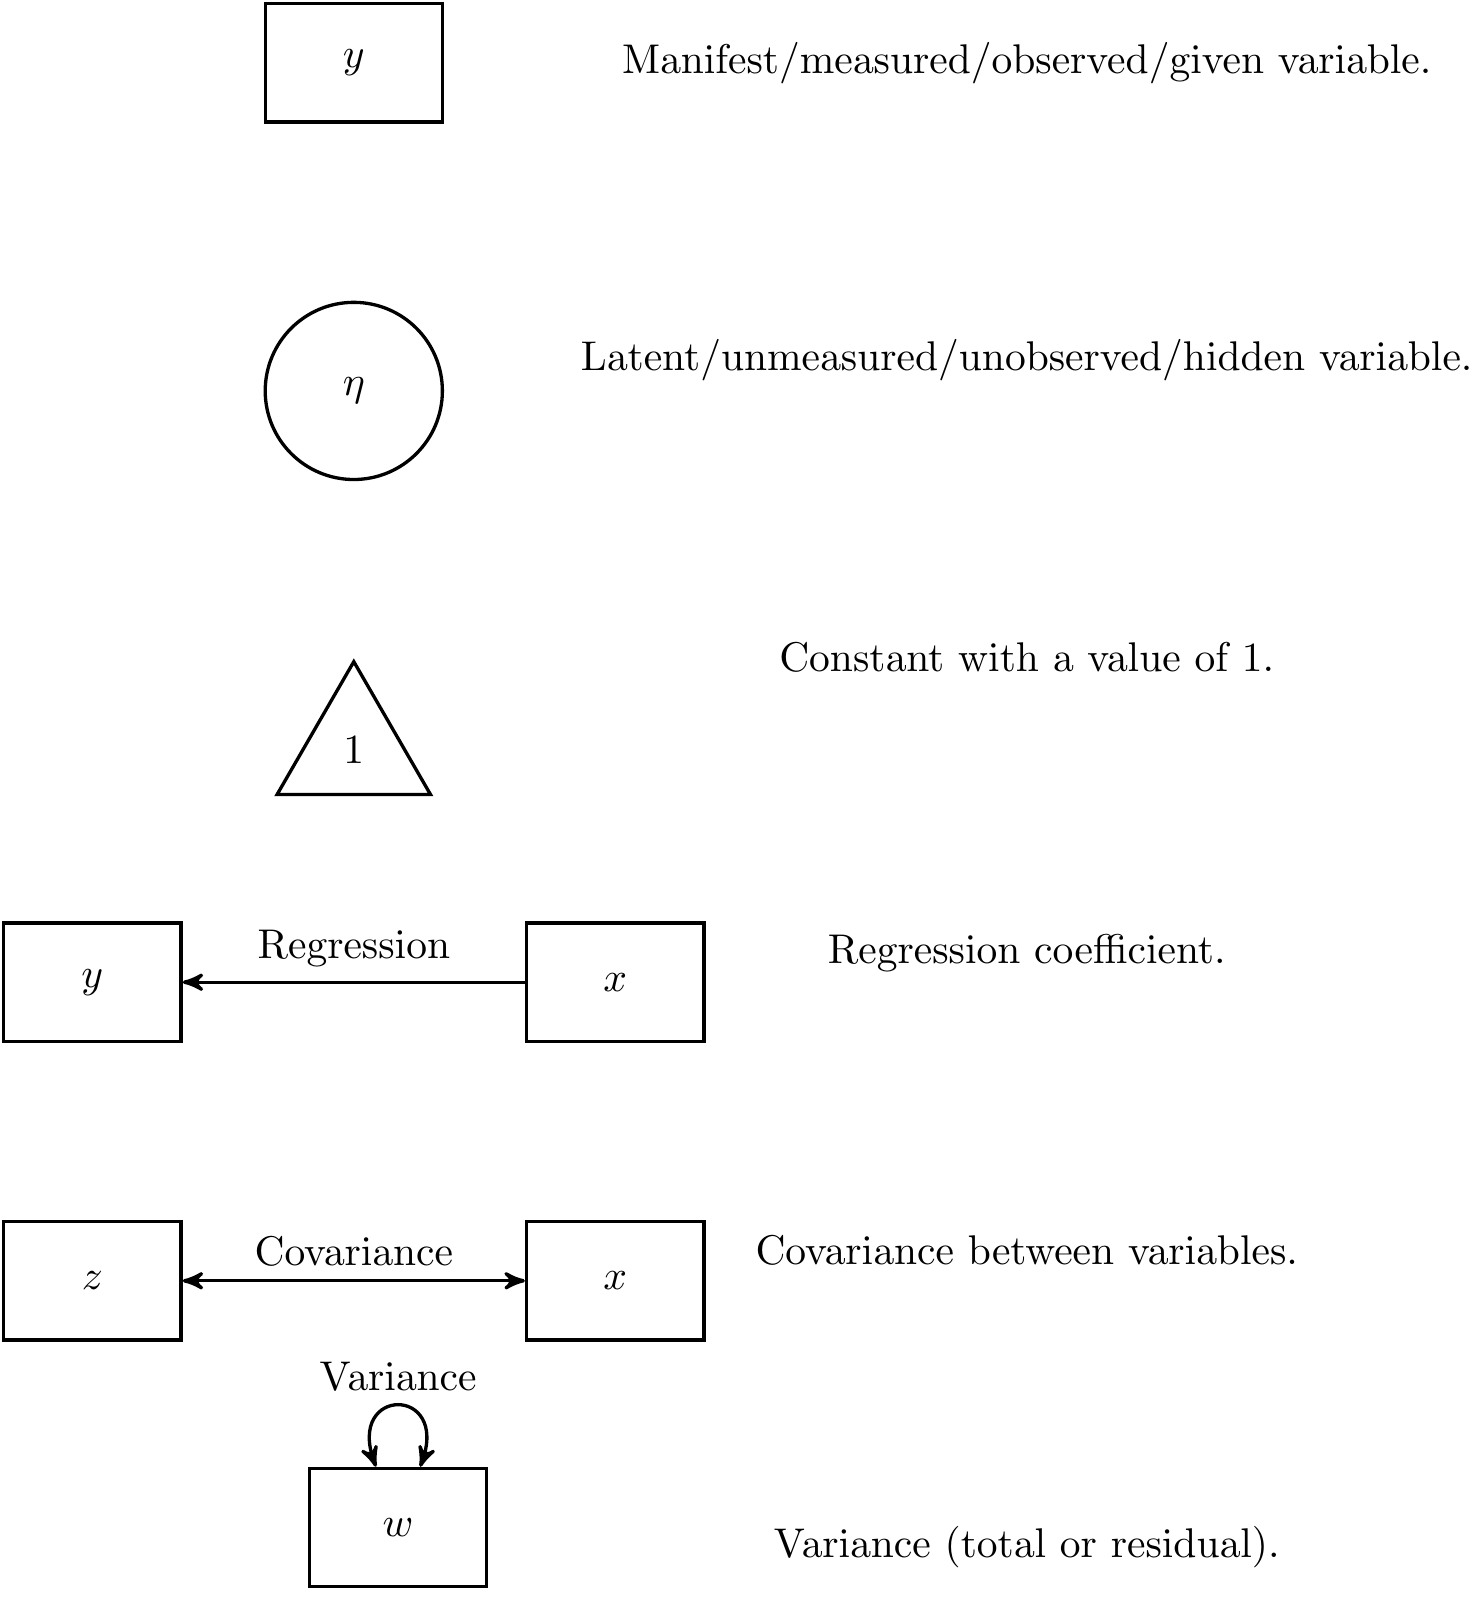
\includegraphics{ramR_notes_files/figure-latex/ram-diagram-01-1.pdf}
\caption{\label{fig:ram-diagram-01}Path Diagram Elements}
\end{figure}

\begin{figure}
\centering
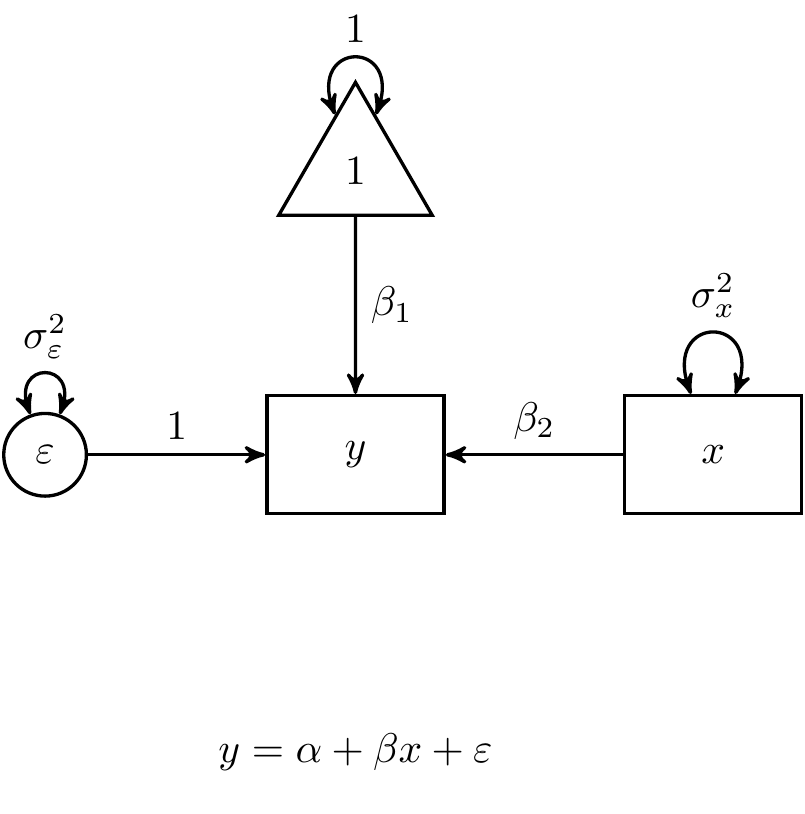
\includegraphics{ramR_notes_files/figure-latex/ram-diagram-02-1.pdf}
\caption{\label{fig:ram-diagram-02}Two-Variable Regression Model}
\end{figure}

\begin{figure}
\centering
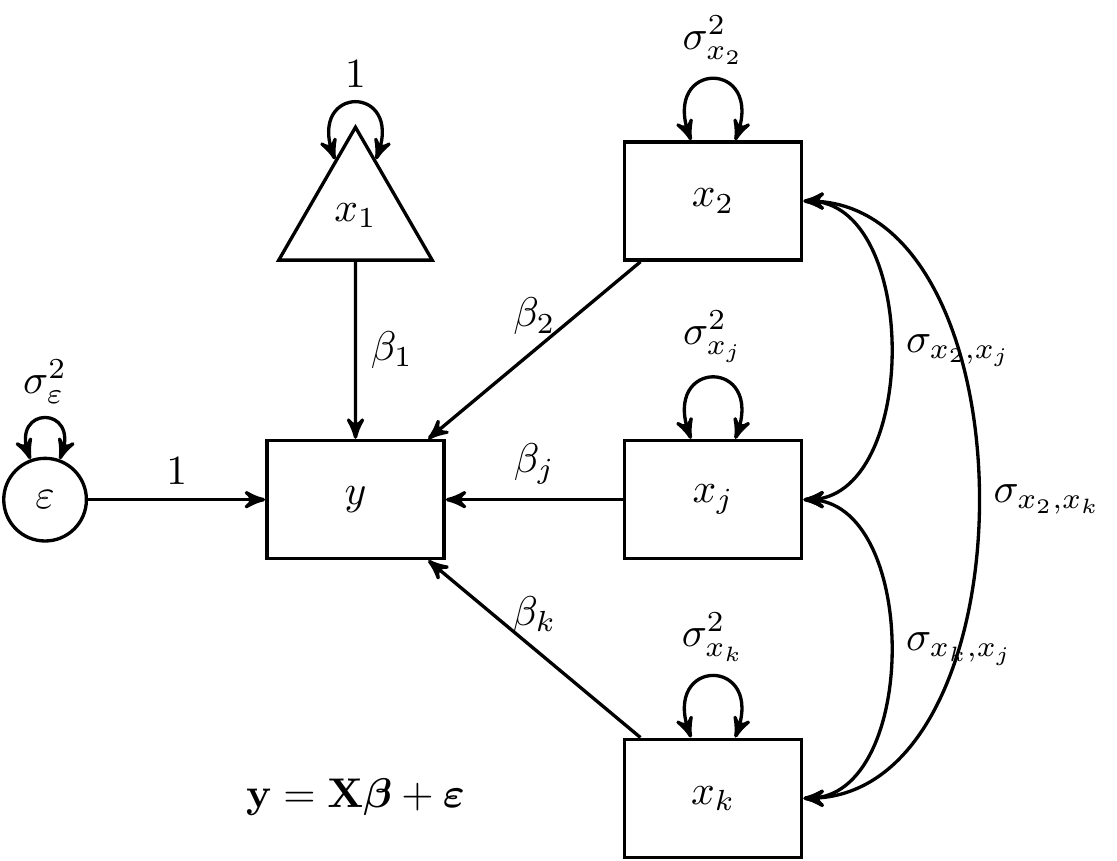
\includegraphics{ramR_notes_files/figure-latex/ram-diagram-03-1.pdf}
\caption{\label{fig:ram-diagram-03}\(k\)-Variable Regression Model}
\end{figure}

\begin{figure}
\centering
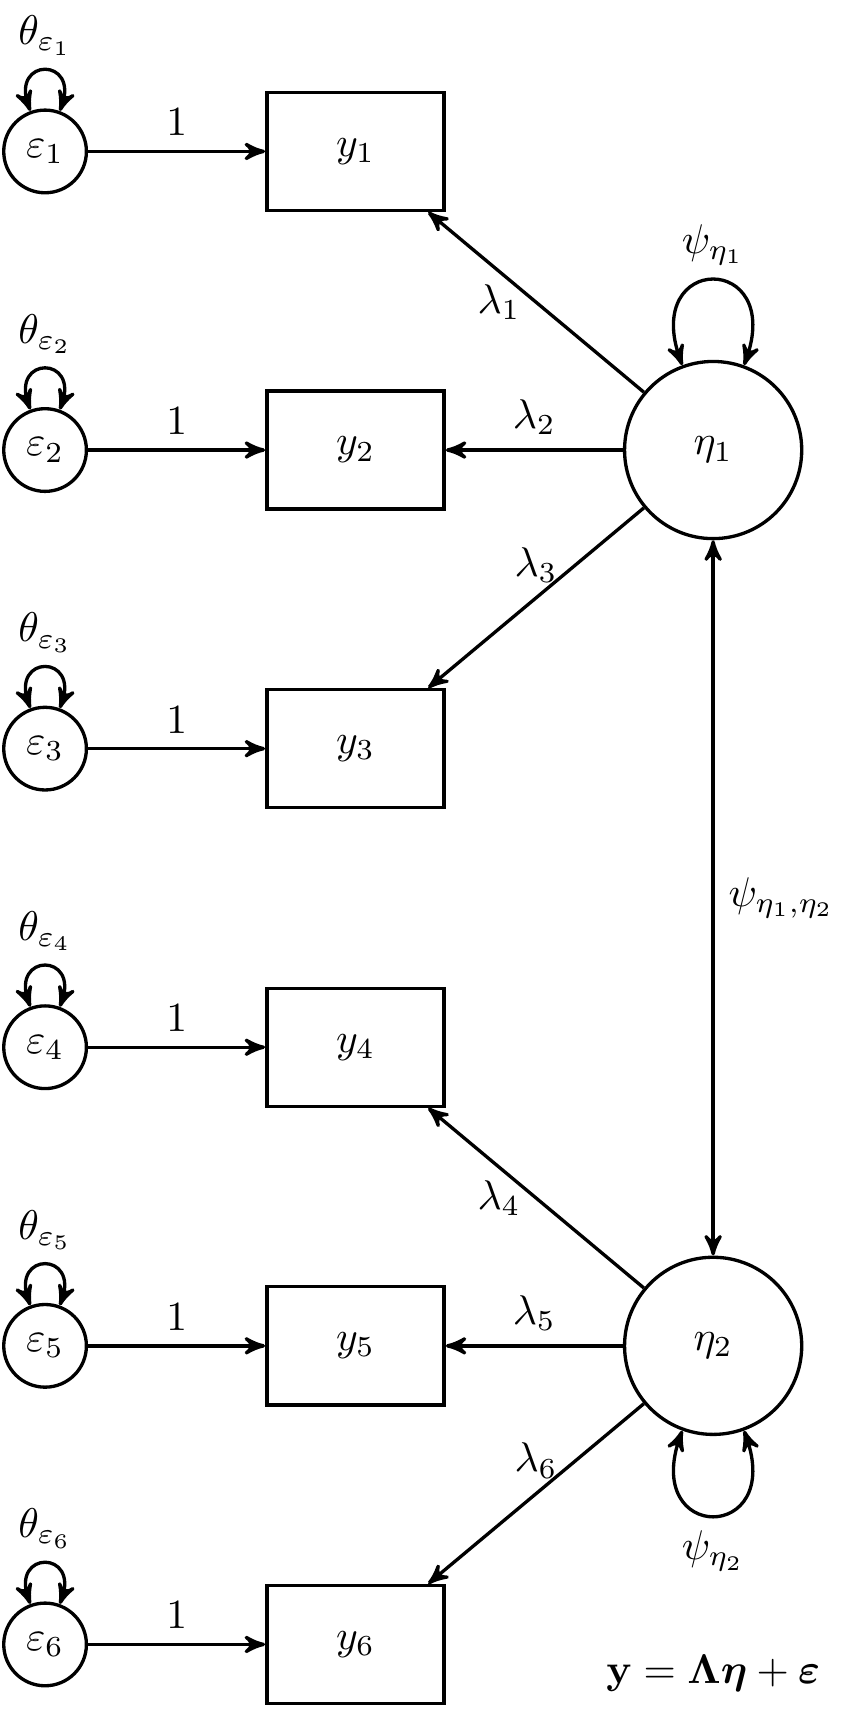
\includegraphics{ramR_notes_files/figure-latex/ram-diagram-04-1.pdf}
\caption{\label{fig:ram-diagram-04}Two-Factor Confirmatory Factor Analysis Model}
\end{figure}

\hypertarget{ram-t}{%
\chapter{\texorpdfstring{Student's \(t\)-test}{Student's t-test}}\label{ram-t}}

In this section,
the Student's \(t\)-test is presented as a structural equation model
using the RAM notation.
Let \(y\) be a continuous dependent variable,
\(x\) be a dichotomous independent variable
\(\left( x = \{0, 1\} \right)\),
and \(\varepsilon\) be the stochastic error term
with mean 0 and constant variance of \(\sigma_{\varepsilon}^{2}\)
across the values of \(x\).
The associations of the variables are given by

\begin{equation*}
  y
  =
  \alpha + \beta x + \varepsilon
\end{equation*}

\noindent where

\begin{itemize}
\tightlist
\item
  \(\alpha\) is the expected value of \(y\) when \(x = 0\)
\item
  \(\beta\) is the unit change in \(y\) for unit change in \(x\)
\item
  \(\alpha + \beta\) is the expected value of \(y\) when \(x = 1\)
\end{itemize}

\begin{figure}
\centering
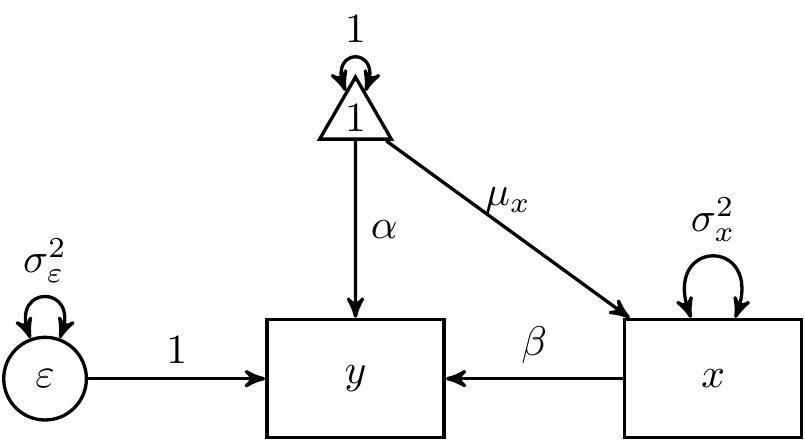
\includegraphics{ramR_notes_files/figure-latex/ram-t-01-1.pdf}
\caption{\label{fig:ram-t-01}Student's \(t\)-test}
\end{figure}

\hypertarget{symbolic}{%
\section{Symbolic}\label{symbolic}}

Let \(\left\{ y, x, \varepsilon \right\}\) be the variables of interest.

\begin{align*}\mathbf{A} &=\left( \begin{array}{ccc} 0 & \beta  & 1 \\ 0 & 0 & 0 \\ 0 & 0 & 0 \end{array} \right)\end{align*}

\begin{align*}\mathbf{S} &=\left( \begin{array}{ccc} 0 & 0 & 0 \\ 0 & \sigma  _{x} ^{2} & 0 \\ 0 & 0 & \sigma  _{\varepsilon } ^{2} \end{array} \right)\end{align*}

\begin{align*}\mathbf{C} &=\left( \mathbf{I} - \mathbf{A} \right)^{-1} \mathbf{S} \left[ \left( \mathbf{I} - \mathbf{A} \right)^{-1} \right]^{\mathsf{T}} \\\\ &=\mathbf{E} \mathbf{S} \mathbf{E}^{\mathsf{T}} \\\\ &=\left( \begin{array}{ccc} 1 & \beta  & 1 \\ 0 & 1 & 0 \\ 0 & 0 & 1 \end{array} \right)\left( \begin{array}{ccc} 0 & 0 & 0 \\ 0 & \sigma  _{x} ^{2} & 0 \\ 0 & 0 & \sigma  _{\varepsilon } ^{2} \end{array} \right)\left( \begin{array}{ccc} 1 & \beta  & 1 \\ 0 & 1 & 0 \\ 0 & 0 & 1 \end{array} \right)^{\mathsf{T}}\\ &=\left( \begin{array}{ccc} \sigma  _{x} ^{2} \beta  ^{2} + \sigma  _{\varepsilon } ^{2} & \beta  \sigma  _{x} ^{2} & \sigma  _{\varepsilon } ^{2} \\ \sigma  _{x} ^{2} \beta  & \sigma  _{x} ^{2} & 0 \\ \sigma  _{\varepsilon } ^{2} & 0 & \sigma  _{\varepsilon } ^{2} \end{array} \right)\end{align*}

\begin{align*}\mathbf{F} &=\left( \begin{array}{ccc} 1 & 0 & 0 \\ 0 & 1 & 0 \end{array} \right)\end{align*}

\begin{align*}\mathbf{M} &=\mathbf{F} \left( \mathbf{I} - \mathbf{A} \right)^{-1} \mathbf{S} \left[ \left( \mathbf{I} - \mathbf{A} \right)^{-1} \right]^{\mathsf{T}} \mathbf{F}^{\mathsf{T}}\\ &=\mathbf{F} \mathbf{E} \mathbf{S} \mathbf{E}^{\mathsf{T}} \mathbf{F}^{\mathsf{T}} \\\\ &=\mathbf{F} \mathbf{C} \mathbf{F}^{\mathsf{T}} \\\\ &=\left( \begin{array}{ccc} 1 & 0 & 0 \\ 0 & 1 & 0 \end{array} \right)\left( \begin{array}{ccc} \sigma  _{x} ^{2} \beta  ^{2} + \sigma  _{\varepsilon } ^{2} & \beta  \sigma  _{x} ^{2} & \sigma  _{\varepsilon } ^{2} \\ \sigma  _{x} ^{2} \beta  & \sigma  _{x} ^{2} & 0 \\ \sigma  _{\varepsilon } ^{2} & 0 & \sigma  _{\varepsilon } ^{2} \end{array} \right)\left( \begin{array}{ccc} 1 & 0 & 0 \\ 0 & 1 & 0 \end{array} \right)^{\mathsf{T}} \\\\ &=\left( \begin{array}{cc} \sigma  _{x} ^{2} \beta  ^{2} + \sigma  _{\varepsilon } ^{2} & \beta  \sigma  _{x} ^{2} \\ \sigma  _{x} ^{2} \beta  & \sigma  _{x} ^{2} \end{array} \right)\end{align*}

\begin{align*}\mathbf{v} &=\left( \mathbf{I} - \mathbf{A} \right)^{-1} \mathbf{u}\\ &=\left[\left( \begin{array}{ccc} 1 & 0 & 0 \\ 0 & 1 & 0 \\ 0 & 0 & 1 \end{array} \right)-\left( \begin{array}{ccc} 0 & \beta  & 1 \\ 0 & 0 & 0 \\ 0 & 0 & 0 \end{array} \right)\right]^{\mathsf{-1}}\left( \begin{array}{c} \alpha  \\ \mu  _{x} \\ 0 \end{array} \right)\\ &=\left( \begin{array}{c} \alpha  + \beta  \mu  _{x} \\ \mu  _{x} \\ 0 \end{array} \right)\end{align*}

\begin{align*}\mathbf{u} &=\left( \mathbf{I} - \mathbf{A} \right) \mathbf{v}\\ &=\left[\left( \begin{array}{ccc} 1 & 0 & 0 \\ 0 & 1 & 0 \\ 0 & 0 & 1 \end{array} \right)-\left( \begin{array}{ccc} 0 & \beta  & 1 \\ 0 & 0 & 0 \\ 0 & 0 & 0 \end{array} \right)\right]\left( \begin{array}{c} \alpha  + \beta  \mu  _{x} \\ \mu  _{x} \\ 0 \end{array} \right)\\ &=\left( \begin{array}{c} \alpha  \\ \mu  _{x} \\ 0 \end{array} \right)\end{align*}

\begin{align*}\mathbf{g} &=\mathbf{F} \left( \mathbf{I} - \mathbf{A} \right)^{-1} \mathbf{u}\\ &=\left[\left( \begin{array}{ccc} 1 & 0 & 0 \\ 0 & 1 & 0 \\ 0 & 0 & 1 \end{array} \right)-\left( \begin{array}{ccc} 0 & \beta  & 1 \\ 0 & 0 & 0 \\ 0 & 0 & 0 \end{array} \right)\right]^{-1}\left( \begin{array}{c} \alpha  \\ \mu  _{x} \\ 0 \end{array} \right)\\ &=\left( \begin{array}{c} \alpha  + \beta  \mu  _{x} \\ \mu  _{x} \end{array} \right)\end{align*}

\hypertarget{using-the-ramr-package}{%
\subsection{\texorpdfstring{Using the \texttt{ramR} Package}{Using the ramR Package}}\label{using-the-ramr-package}}

\begin{Shaded}
\begin{Highlighting}[]
\NormalTok{A}
\end{Highlighting}
\end{Shaded}

\begin{verbatim}
##      [,1] [,2]   [,3]
## [1,] "0"  "beta" "1" 
## [2,] "0"  "0"    "0" 
## [3,] "0"  "0"    "0"
\end{verbatim}

\begin{Shaded}
\begin{Highlighting}[]
\NormalTok{S}
\end{Highlighting}
\end{Shaded}

\begin{verbatim}
##      [,1] [,2]         [,3]                 
## [1,] "0"  "0"          "0"                  
## [2,] "0"  "sigma[x]^2" "0"                  
## [3,] "0"  "0"          "sigma[varepsilon]^2"
\end{verbatim}

\begin{Shaded}
\begin{Highlighting}[]
\NormalTok{u}
\end{Highlighting}
\end{Shaded}

\begin{verbatim}
##      [,1]   
## [1,] "alpha"
## [2,] "mu[x]"
## [3,] "0"
\end{verbatim}

\begin{Shaded}
\begin{Highlighting}[]
\NormalTok{filter}
\end{Highlighting}
\end{Shaded}

\begin{verbatim}
##      [,1] [,2] [,3]
## [1,]    1    0    0
## [2,]    0    1    0
\end{verbatim}

The covariance expectations
can be symbolically derived using the \texttt{ramR::C\_sym()} function.

\begin{Shaded}
\begin{Highlighting}[]
\NormalTok{ramR}\SpecialCharTok{::}\FunctionTok{C\_sym}\NormalTok{(A, S)}
\end{Highlighting}
\end{Shaded}

\begin{verbatim}
## {{sigma[x]^2*beta^2+sigma[varepsilon]^2,                       beta*sigma[x]^2,                   sigma[varepsilon]^2},
##  {                      sigma[x]^2*beta,                            sigma[x]^2,                                     0},
##  {                  sigma[varepsilon]^2,                                     0,                   sigma[varepsilon]^2}}
\end{verbatim}

\begin{equation*}\mathbf{C} =\left( \begin{array}{ccc} \sigma  _{x} ^{2} \beta  ^{2} + \sigma  _{\varepsilon } ^{2} & \beta  \sigma  _{x} ^{2} & \sigma  _{\varepsilon } ^{2} \\ \sigma  _{x} ^{2} \beta  & \sigma  _{x} ^{2} & 0 \\ \sigma  _{\varepsilon } ^{2} & 0 & \sigma  _{\varepsilon } ^{2} \end{array} \right)\end{equation*}

The covariance expectations for the observed variables
can be symbolically derived using the \texttt{ramR::M\_sym()} function.

\begin{Shaded}
\begin{Highlighting}[]
\NormalTok{ramR}\SpecialCharTok{::}\FunctionTok{M\_sym}\NormalTok{(A, S, filter)}
\end{Highlighting}
\end{Shaded}

\begin{verbatim}
## {{sigma[x]^2*beta^2+sigma[varepsilon]^2,                       beta*sigma[x]^2},
##  {                      sigma[x]^2*beta,                            sigma[x]^2}}
\end{verbatim}

\begin{equation*}\mathbf{M} =\left( \begin{array}{cc} \sigma  _{x} ^{2} \beta  ^{2} + \sigma  _{\varepsilon } ^{2} & \beta  \sigma  _{x} ^{2} \\ \sigma  _{x} ^{2} \beta  & \sigma  _{x} ^{2} \end{array} \right)\end{equation*}

The mean expectations
can be symbolically derived using the \texttt{ramR::v\_sym()} function.

\begin{Shaded}
\begin{Highlighting}[]
\NormalTok{ramR}\SpecialCharTok{::}\FunctionTok{v\_sym}\NormalTok{(A, u)}
\end{Highlighting}
\end{Shaded}

\begin{verbatim}
## {{alpha+beta*mu[x]},
##  {           mu[x]},
##  {               0}}
\end{verbatim}

\begin{equation*}\mathbf{v} =\left( \begin{array}{c} \alpha  + \beta  \mu  _{x} \\ \mu  _{x} \\ 0 \end{array} \right)\end{equation*}

The mean expectations for the observed variables
can be symbolically derived using the \texttt{ramR::g\_sym()} function.

\begin{Shaded}
\begin{Highlighting}[]
\NormalTok{ramR}\SpecialCharTok{::}\FunctionTok{g\_sym}\NormalTok{(A, u, filter)}
\end{Highlighting}
\end{Shaded}

\begin{verbatim}
## {{alpha+beta*mu[x]},
##  {           mu[x]}}
\end{verbatim}

\begin{equation*}\mathbf{g} =\left( \begin{array}{c} \alpha  + \beta  \mu  _{x} \\ \mu  _{x} \end{array} \right)\end{equation*}

\hypertarget{numerical-example}{%
\section{Numerical Example}\label{numerical-example}}

\begin{Shaded}
\begin{Highlighting}[]
\FunctionTok{head}\NormalTok{(df)}
\end{Highlighting}
\end{Shaded}

\begin{verbatim}
##            y x
## 1  1.3709584 0
## 2 -0.5646982 0
## 3  0.3631284 0
## 4  0.6328626 0
## 5  0.4042683 0
## 6 -0.1061245 0
\end{verbatim}

\begin{Shaded}
\begin{Highlighting}[]
\FunctionTok{summary}\NormalTok{(df)}
\end{Highlighting}
\end{Shaded}

\begin{verbatim}
##        y                 x      
##  Min.   :-4.6785   Min.   :0.0  
##  1st Qu.:-0.2622   1st Qu.:0.0  
##  Median : 0.5013   Median :0.5  
##  Mean   : 0.5000   Mean   :0.5  
##  3rd Qu.: 1.2618   3rd Qu.:1.0  
##  Max.   : 5.7839   Max.   :1.0
\end{verbatim}

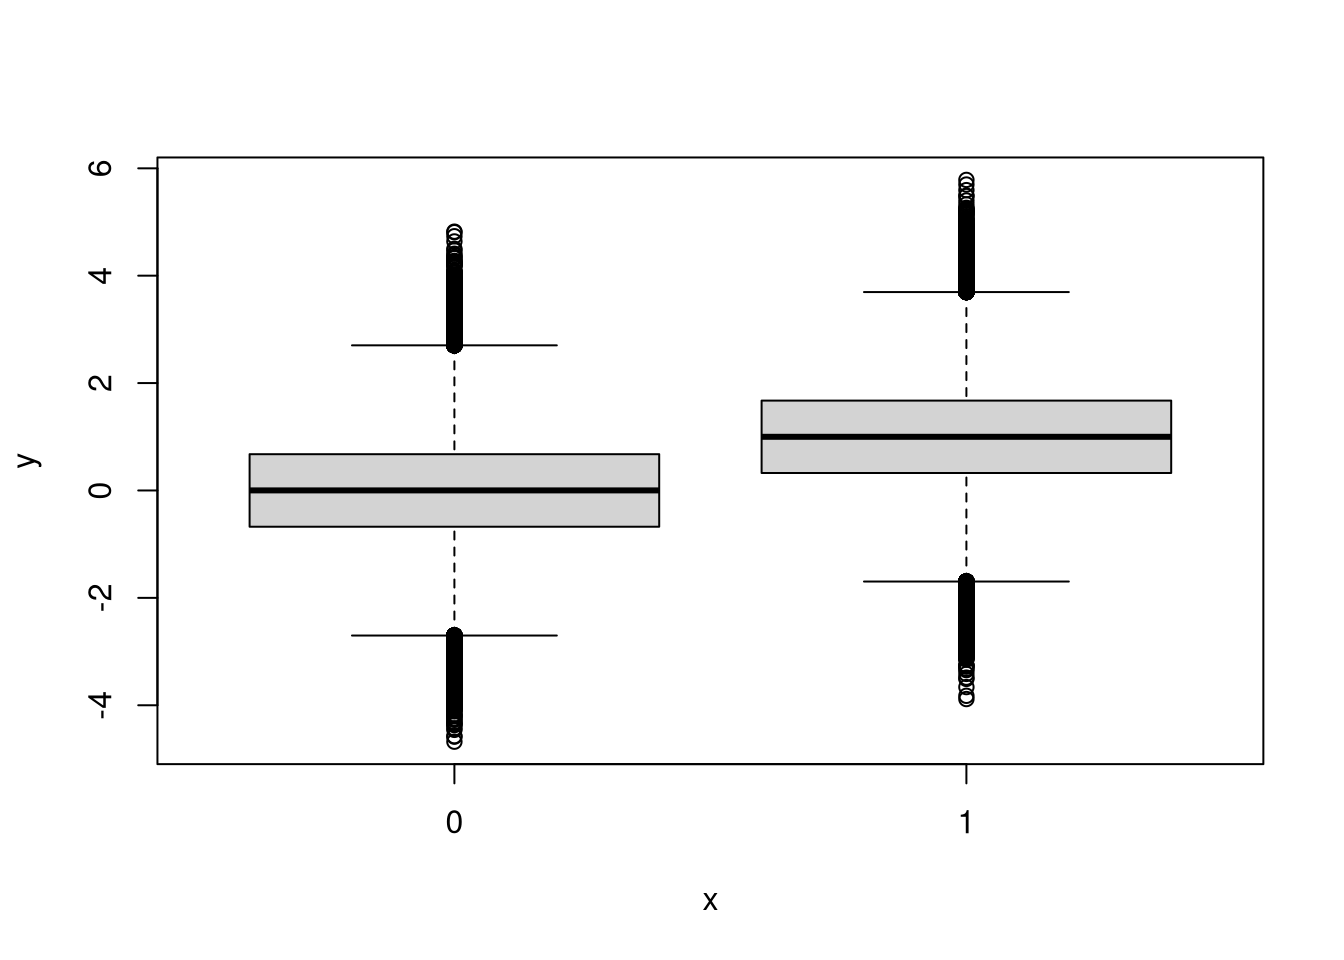
\includegraphics{ramR_notes_files/figure-latex/unnamed-chunk-33-1.pdf} 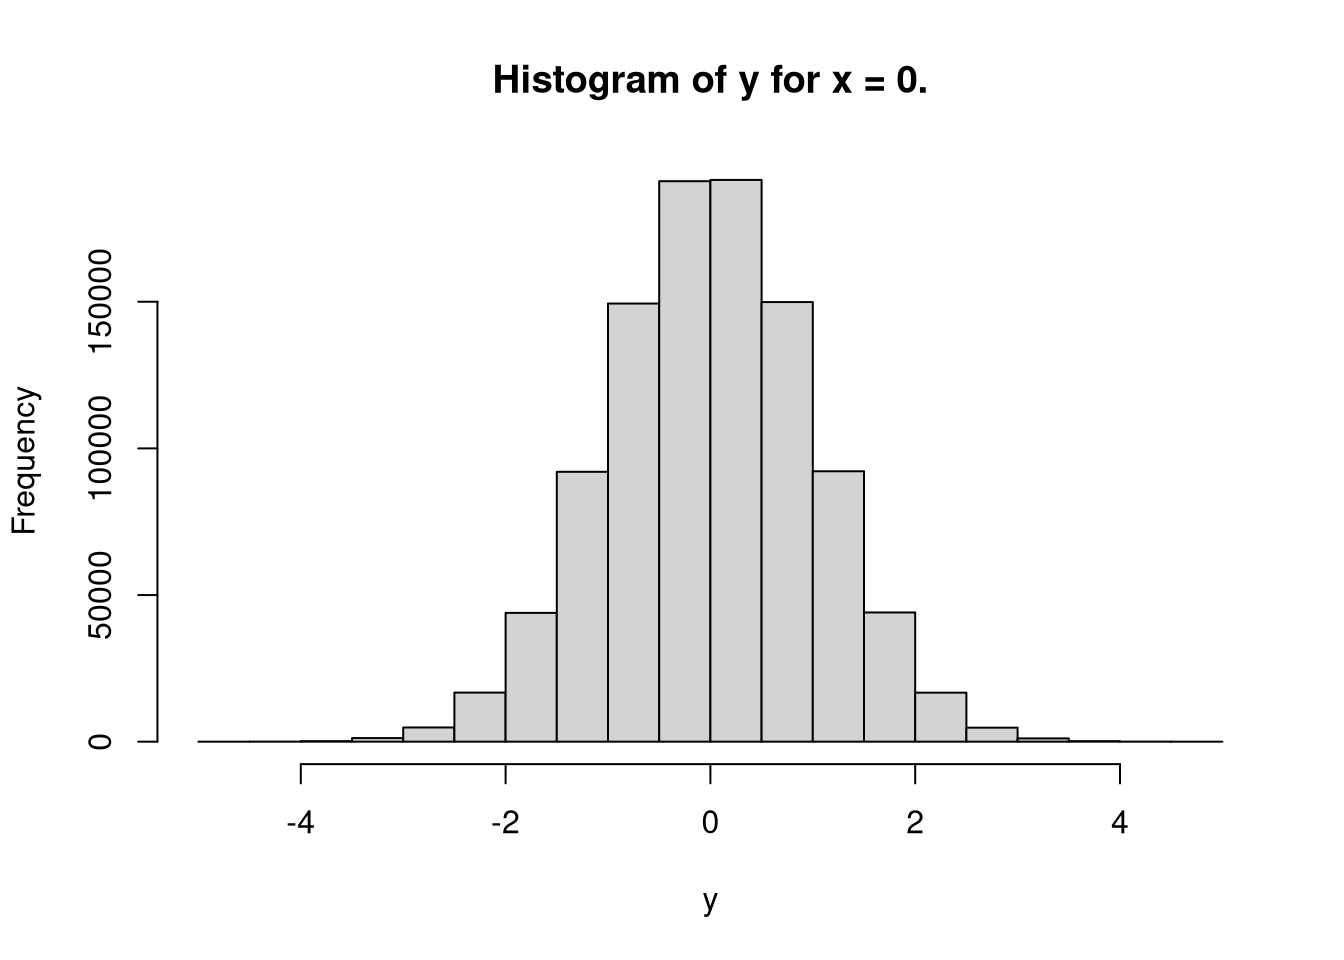
\includegraphics{ramR_notes_files/figure-latex/unnamed-chunk-33-2.pdf} 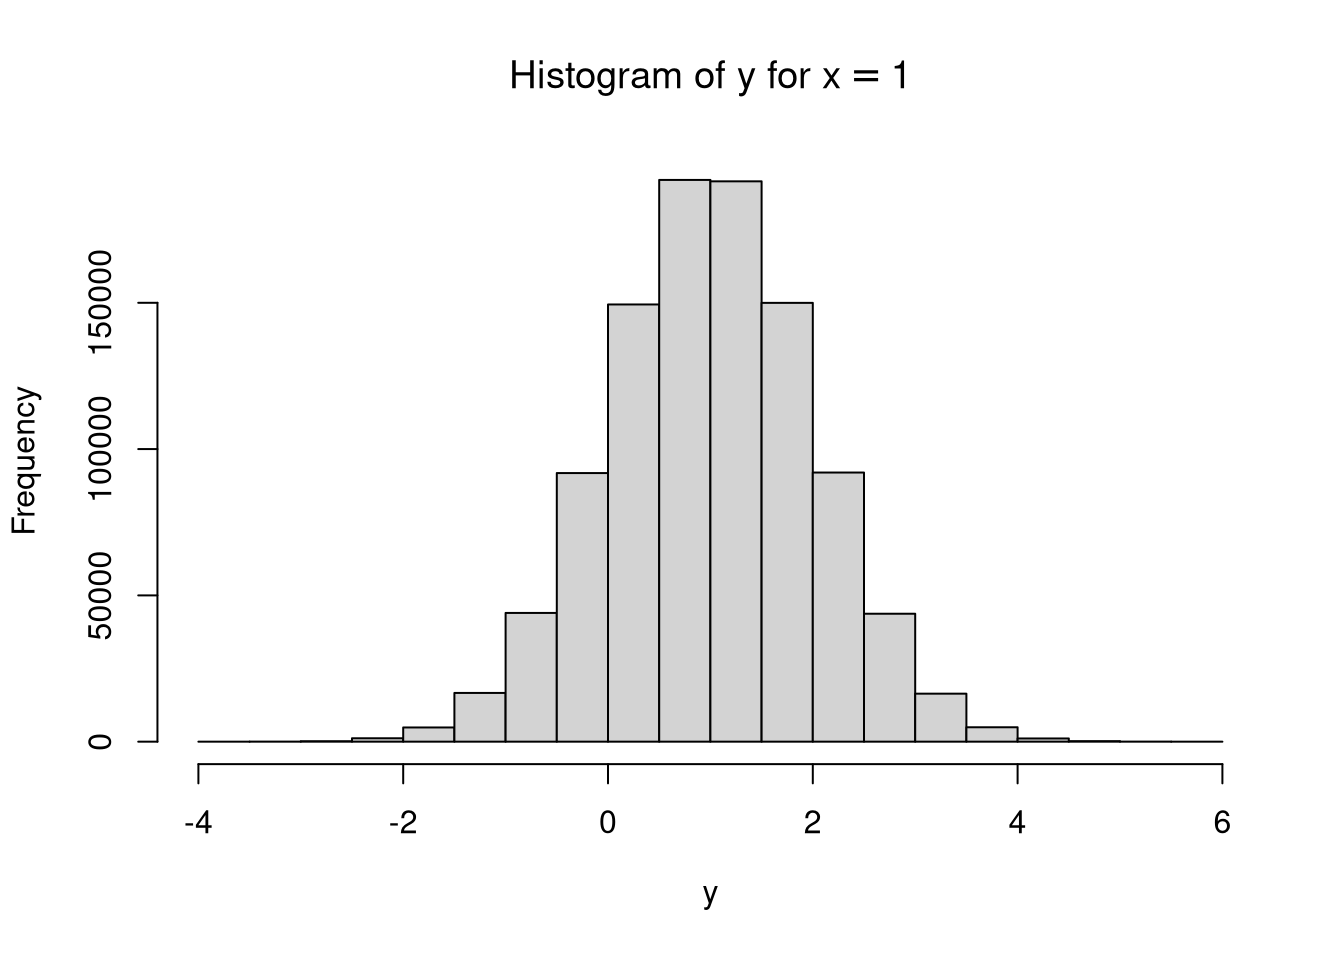
\includegraphics{ramR_notes_files/figure-latex/unnamed-chunk-33-3.pdf}

\begin{Shaded}
\begin{Highlighting}[]
\FunctionTok{t.test}\NormalTok{(y }\SpecialCharTok{\textasciitilde{}}\NormalTok{ x, }\AttributeTok{data =}\NormalTok{ df)}
\end{Highlighting}
\end{Shaded}

\begin{verbatim}
## 
##  Welch Two Sample t-test
## 
## data:  y by x
## t = -706.06, df = 2e+06, p-value < 2.2e-16
## alternative hypothesis: true difference in means is not equal to 0
## 95 percent confidence interval:
##  -1.0016565 -0.9961108
## sample estimates:
## mean in group 0 mean in group 1 
##    0.0005737398    0.9994574009
\end{verbatim}

\begin{Shaded}
\begin{Highlighting}[]
\FunctionTok{summary}\NormalTok{(}\FunctionTok{lm}\NormalTok{(y }\SpecialCharTok{\textasciitilde{}}\NormalTok{ x, }\AttributeTok{data =}\NormalTok{ df))}
\end{Highlighting}
\end{Shaded}

\begin{verbatim}
## 
## Call:
## lm(formula = y ~ x, data = df)
## 
## Residuals:
##     Min      1Q  Median      3Q     Max 
## -4.8838 -0.6745  0.0005  0.6749  4.8195 
## 
## Coefficients:
##              Estimate Std. Error t value Pr(>|t|)    
## (Intercept) 0.0005737  0.0010004   0.574    0.566    
## x           0.9988837  0.0014147 706.057   <2e-16 ***
## ---
## Signif. codes:  0 '***' 0.001 '**' 0.01 '*' 0.05 '.' 0.1 ' ' 1
## 
## Residual standard error: 1 on 1999998 degrees of freedom
## Multiple R-squared:  0.1995, Adjusted R-squared:  0.1995 
## F-statistic: 4.985e+05 on 1 and 1999998 DF,  p-value: < 2.2e-16
\end{verbatim}

\begin{Shaded}
\begin{Highlighting}[]
\NormalTok{model }\OtherTok{\textless{}{-}} \StringTok{"}
\StringTok{  y \textasciitilde{} x}
\StringTok{  y \textasciitilde{} 1}
\StringTok{  x \textasciitilde{} 1}
\StringTok{"}
\NormalTok{fit }\OtherTok{\textless{}{-}}\NormalTok{ lavaan}\SpecialCharTok{::}\FunctionTok{sem}\NormalTok{(model, }\AttributeTok{data =}\NormalTok{ df)}
\NormalTok{lavaan}\SpecialCharTok{::}\FunctionTok{summary}\NormalTok{(fit)}
\end{Highlighting}
\end{Shaded}

\begin{verbatim}
## lavaan 0.6-7 ended normally after 15 iterations
## 
##   Estimator                                         ML
##   Optimization method                           NLMINB
##   Number of free parameters                          5
##                                                       
##   Number of observations                       2000000
##                                                       
## Model Test User Model:
##                                                       
##   Test statistic                                 0.000
##   Degrees of freedom                                 0
## 
## Parameter Estimates:
## 
##   Standard errors                             Standard
##   Information                                 Expected
##   Information saturated (h1) model          Structured
## 
## Regressions:
##                    Estimate  Std.Err  z-value  P(>|z|)
##   y ~                                                 
##     x                 0.999    0.001  706.057    0.000
## 
## Intercepts:
##                    Estimate  Std.Err  z-value  P(>|z|)
##    .y                 0.001    0.001    0.574    0.566
##     x                 0.500    0.000 1414.214    0.000
## 
## Variances:
##                    Estimate  Std.Err  z-value  P(>|z|)
##    .y                 1.001    0.001 1000.000    0.000
##     x                 0.250    0.000 1000.000    0.000
\end{verbatim}

\begin{tabular}{l|l}
\hline
label & parameter\\
\hline
\$\textbackslash{}alpha\$ & 0\\
\hline
\$\textbackslash{}beta\$ & 1\\
\hline
\$\textbackslash{}sigma\textasciicircum{}\{2\}\_\{x\}\$ & 0.25\\
\hline
\$\textbackslash{}sigma\textasciicircum{}\{2\}\_\{\textbackslash{}varepsilon\}\$ & 0.25\\
\hline
\$\textbackslash{}mu\_x\$ & 0.5\\
\hline
\end{tabular}

\hypertarget{using-the-ramr-package-1}{%
\subsection{\texorpdfstring{Using the \texttt{ramR} Package}{Using the ramR Package}}\label{using-the-ramr-package-1}}

\begin{Shaded}
\begin{Highlighting}[]
\NormalTok{A}
\end{Highlighting}
\end{Shaded}

\begin{verbatim}
##   y         x e
## y 0 0.9988837 1
## x 0 0.0000000 0
## e 0 0.0000000 0
\end{verbatim}

\begin{Shaded}
\begin{Highlighting}[]
\NormalTok{S}
\end{Highlighting}
\end{Shaded}

\begin{verbatim}
##   y         x         e
## y 0 0.0000000 0.0000000
## x 0 0.2500001 0.0000000
## e 0 0.0000000 0.2494423
\end{verbatim}

\begin{Shaded}
\begin{Highlighting}[]
\NormalTok{u}
\end{Highlighting}
\end{Shaded}

\begin{verbatim}
##           [,1]
## y 0.0005737398
## x 0.5000000000
## e 0.0000000000
\end{verbatim}

\begin{Shaded}
\begin{Highlighting}[]
\NormalTok{filter}
\end{Highlighting}
\end{Shaded}

\begin{verbatim}
##   y x e
## y 1 0 0
## x 0 1 0
\end{verbatim}

The covariance expectations
can be numerically derived using the \texttt{ramR::C\_num()} function.

\begin{Shaded}
\begin{Highlighting}[]
\NormalTok{ramR}\SpecialCharTok{::}\FunctionTok{C\_num}\NormalTok{(A, S)}
\end{Highlighting}
\end{Shaded}

\begin{verbatim}
##           y         x         e
## y 0.4988845 0.2497210 0.2494423
## x 0.2497210 0.2500001 0.0000000
## e 0.2494423 0.0000000 0.2494423
\end{verbatim}

The covariance expectations for the observed variables
can be numerically derived using the \texttt{ramR::M\_num()} function.

\begin{Shaded}
\begin{Highlighting}[]
\NormalTok{ramR}\SpecialCharTok{::}\FunctionTok{M\_num}\NormalTok{(A, S, filter)}
\end{Highlighting}
\end{Shaded}

\begin{verbatim}
##           y         x
## y 0.4988845 0.2497210
## x 0.2497210 0.2500001
\end{verbatim}

The mean expectations
can be numerically derived using the \texttt{ramR::v\_num()} function.

\begin{Shaded}
\begin{Highlighting}[]
\NormalTok{ramR}\SpecialCharTok{::}\FunctionTok{v\_num}\NormalTok{(A, u)}
\end{Highlighting}
\end{Shaded}

\begin{verbatim}
##           v
## y 0.5000156
## x 0.5000000
## e 0.0000000
\end{verbatim}

The mean expectations for the observed variables
can be numerically derived using the \texttt{ramR::v\_num()} function.

\begin{Shaded}
\begin{Highlighting}[]
\NormalTok{ramR}\SpecialCharTok{::}\FunctionTok{g\_num}\NormalTok{(A, u, filter)}
\end{Highlighting}
\end{Shaded}

\begin{verbatim}
##           g
## y 0.5000156
## x 0.5000000
\end{verbatim}

  \bibliography{book.bib,packages.bib}

\end{document}
